\documentclass[a4paper]{article}
\usepackage{amssymb}
\usepackage{amsmath}
\usepackage{hyperref}
\usepackage[italian]{cleveref}
\usepackage[italian]{babel}
%\usepackage[nomarkers]{endfloat}
\usepackage{graphicx}
\usepackage[margin=3cm]{geometry}
\usepackage{mathtools}
\usepackage{subcaption}
\usepackage[table]{xcolor}
%\renewcommand{\efloatseparator}{\mbox{}}
%\renewcommand{\efloatendlist}{\mbox{}}
\newenvironment{eqsys}{\begin{equation}\begin{dcases}}{\end{dcases}\end{equation}}

\DeclareMathOperator*{\sca}{\textrm{sca}}
\title{Progetto Controlli Automatici T \\ 1C - Controllo del posizionamento di un link flessibile}
\author{Riccardo Corradini \and Luigi di Nuzzo \and Kevin Michael Frick \and Davide Ragazzini \and Antony Zappacosta}
\begin{document}
\maketitle
\tableofcontents
\clearpage
\section{Descrizione e requisiti del sistema}
Nella nuova applicazione della azienda che commissiona il progetto si prevede di utilizzare una struttura meccanica particolarmente leggera. 
Questa però presenta il problema di una flessibilità non trascurabile intrinseca nei componenti meccanici utilizzati. 
Ciò rende difficile il posizionamento dell’estremità non attuata in una posizione fissa desiderata.
\subsection{Modello e linearizzazione}
L’intera struttura in questione è modellizzata da \cref{eqn:model} ed è schematizzata come in \cref{fig:sys_schem}.
\begin{eqsys}       
    \label{eqn:model}
    \dot{x_1}  =  f_1 (x_1, x_2, x_3, x_4)  =  x_2 \\
    \dot{x_2}  =  f_2 (x_1, x_2, x_3, x_4)  =  \frac{-M g L \sin (x_1) - K (x_1 - x_3) - \rho (x_2 - x_4)}{J} \\
    \dot{x_3}  =  f_3 (x_1, x_2, x_3, x_4)  =  x_4 \\
    \dot{x_4}  =  f_4 (x_1, x_2, x_3, x_4) + g(u)  =  \frac{K(x_1 - x_2) + \rho (x_2 - x_4) + u}{I}\\
    y  =  f_y (x_1, x_2, x_3, x_4)  =  x_1
\end{eqsys}
\begin{figure}[h!]
    \centering
 \begin{subfigure}{0.45\textwidth}
    \centering
    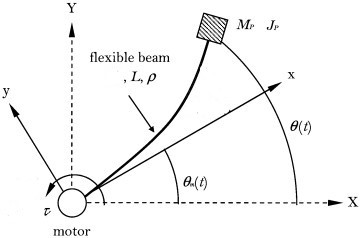
\includegraphics[width=\textwidth]{schematic.png}
    \caption{Schema del modello fisico del sistema.}
    \label{fig:sys_schem}
 \end{subfigure}
 ~
 \begin{subfigure}{0.45\textwidth}
    \centering
    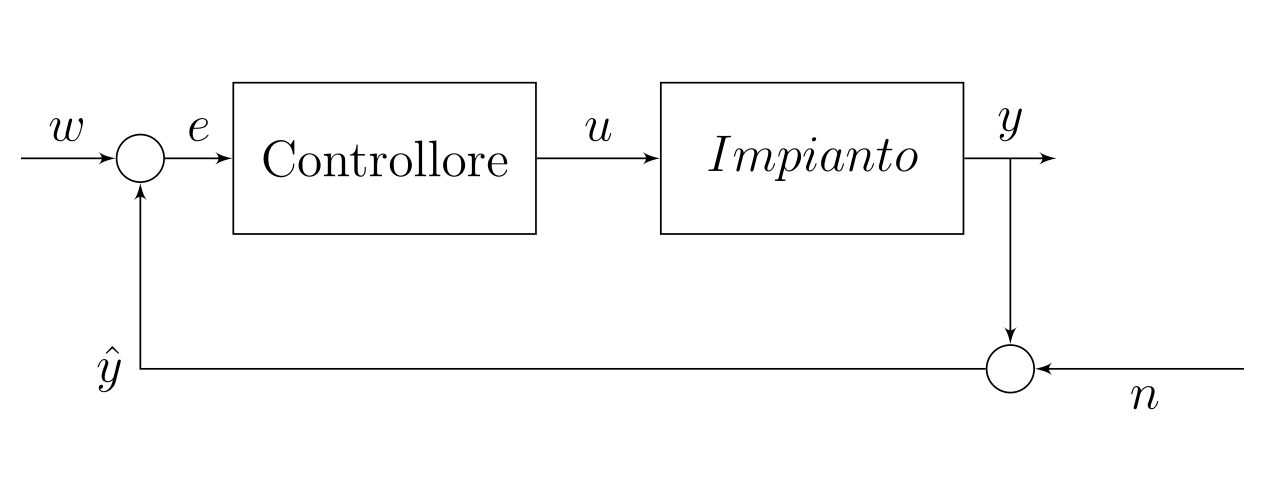
\includegraphics[width=\textwidth]{control_sys.png}
    \caption{Schema di controllo del sistema linearizzato.}
    \label{fig:sys_cont}
 \end{subfigure}
\end{figure}
La variabile $\theta$ in \cref{fig:sys_schem} viene descritta dallo stato $x_1$ e rappresenta l’angolo rispetto ad un piano di riferimento fisso che la massa concentrata del link traccia nel suo moto. $\theta_m$ (nelle equazioni $x_3$) rappresenta l’angolo di rotazione del motore, il cui input $u$ al sistema è la coppia applicata $\tau_m$. $K, \rho, L, M_p, J_p, I$ sono rispettivamente: la costante elastica del link, il suo coefficiente di attrito dinamico, la lunghezza, la massa concentrata sull’estremità non attuata, il momento d’inerzia della stessa massa e il momento d’inerzia del link equivalente visto dal punto di vista del motore.
Ai fini dello sviluppo del controllo dell’impianto si vuole ottenere la struttura in \cref{fig:sys_cont}.

Come prima analisi il sistema non lineare deve essere considerato nell’intorno di un punto di equilibrio, i cui valori $(\bar{x}, \bar{u})$ sono definiti nella \cref{table:ref_val} e linearizzato nello stesso intorno.


{\begin{table}[h]

    \centering 

    \rowcolors{1}{gray!10}{gray!20}
    \begin{tabular}{| c | c || c | c |}
        
        $K$ & 3 &
        $\rho$ & 0.2 \\
        $L$ & 1 &
        $I$ & 0.01 \\
        $J_p$ & 0.02 &
        $M_p$ & 0.06 \\
        $\omega_n$ & 200 &
        $A_n$ & 0.05 \\
        $B_n$ & 20 &
        $h\%$ & 1 \\
        $T_{a_{h^\%}}$ & 0.8 &
        $W$ & $5^\circ$ \\
        $T_{a_o}$ & 0.4 &
        $\bar{u}$  & $M_p g L \sin(\bar{x_1})$ \\
        $\bar{x_1}$  & $\frac{\pi}{2}$ &
        $\bar{x_2}$  & 0 \\
        $\bar{x_3}$  &$\frac{\bar{u}}{K} + \bar{x_1}$ &
        $\bar{x_4}$  & 0
        
        
    \end{tabular}
    \caption{Specifiche del sistema.}
        \label{table:ref_val}
\end{table}
}
\begin{eqsys}       
        \nabla f_1  = (0, 1, 0, 0) \\
        \nabla f_2  = \frac{1}{J_p} (-M_p g L \cos(x_1) - K, - \rho, K, \rho) \\
        \nabla f_3  =  (0, 0, 0, 1)\\
        \nabla f_4  =  \frac{1}{I} (K, \rho, -K, -\rho) \\
        \nabla f_y  =  (1, 0, 0, 0)  \\
        \frac{dg}{du}  =  \frac{1}{I}
        \label{eqn:linearization_calc}
    \end{eqsys}

\begin{equation}
    \label{eqn:linearization}
A = \begin{pmatrix}0 & 1 & 0 & 0 \\
    -K/J_p & -\rho/J_p & K/J_p & \rho/J_p \\
    0    &   0    &   0    &   1\\
    K/I  & \rho/I & -K/I &-\rho/I
\end{pmatrix};
B = (0, 0, 0, \frac{1}{I})^T;
C = (1, 0, 0, 0);
D = (0);
\end{equation}

Il modello nella \cref{eqn:model} è stato quindi linearizzato nell’intorno di $(\bar{x}, \bar{u})$ servendosi della \cref{eqn:linearization_calc} ottenendo la \cref{eqn:linearization}.
È necessario poi passare dalla rappresentazione nello spazio degli stati al dominio di Laplace utilizzando la trasformata di Laplace, ottenendo la funzione di trasferimento nella \cref{eqn:G}.

\begin{equation}
    \label{eqn:G}
    G(s) = \frac{1000 (s+15)}{s^2 (s^2 + 30s + 450)}
\end{equation}

Per l’applicazione che l’azienda ha in mente si devono rispettare per il sistema linearizzato determinate caratteristiche:
\begin{enumerate}
    \item Errore a regime nullo con riferimento a gradino con ampiezza $w(t) = W \sca(t)$.
    \item Per garantire una certa robustezza del sistema si deve avere un margine di fase $\phi_m \geq 45^\circ$.
    \item Il sistema può accettare una sovraelongazione percentuale al massimo dell’1\% : $S\% \leq 1\%$.
    \item Tempo di assestamento all'1\% $T_{a1} = 0.8$ (opzionalmente 0.4).
    \item Abbattimento del rumore di 20 volte.
\end{enumerate}

Il rumore si fa sentire a $\omega_n > 200\hspace{0.5em} rad/s$ con ampiezza $A_n = 0.05$.
    
Dopo aver definito i parametri del sistema, calcolato le matrici linearizzate e la funzione di trasferimento, si definisce su MATLAB l’intervallo di frequenze che sarà mostrato nel diagramma di Bode: $\omega \in [10^{-2}, 10^5]$.

\begin{figure}[h!]
    \centering
    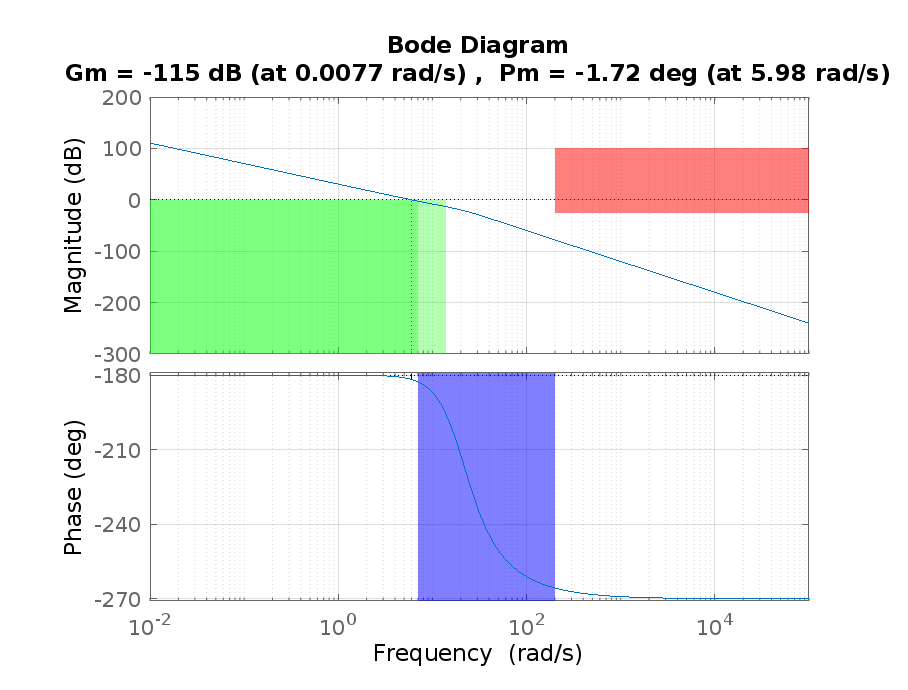
\includegraphics[width=0.8\textwidth]{bode_G}
    \caption{Diagramma di Bode del sistema in anello aperto}
    \label{fig:bode_G}
\end{figure}

\subsection{Requisiti sul margine di fase e sulla pulsazione critica}
Il requisito sulla sovraelongazione si traduce in un requisito sul margine di fase che è maggiore di quello specificato, indicato nella \cref{eqn:phim}.
Tuttavia, durante la sintesi del controllore si è notato che anche non rispettando questo requisito è possibile avere un sistema che rispetti le specifiche di sovraelongazione e abbia un tempo di assestamento ottimale.
Nei diagrammi di Bode la fase proibita è indicata in blu.

\begin{equation}
    \xi = \sqrt{\frac{\log(S_{max})^2}{(\pi^2+\log(S_{max})^2)}} \approx 0.826
    \label{eqn:xi}
\end{equation}

\begin{equation}
    \phi_m \approx \xi \cdot 100 \approx 83^\circ
    \label{eqn:phim}
\end{equation}

Il requisito sul tempo di assestamento si traduce invece in un requisito sulla pulsazione critica, che deve essere maggiore di una certa soglia indicata nella \cref{eqn:omega_c}.
Questa soglia è stata rispettata durante la sintesi del regolatore. 
Nei diagrammi di Bode le "zone proibite" che non rispettano i requisiti sono indicate in verde; le specifiche ottimali usano un colore meno intenso.
\begin{equation}
    \omega_c \gtrsim \frac{460}{\phi_m T_a} \approx 7 (\approx 14 \textrm{ per le specifiche ottimali})
    \label{eqn:omega_c}
\end{equation}

\section{Progetto del regolatore}

Per avere errore a regime nullo è necessario che $L(s)$ abbia un polo nell'origine, ma $G(s)$ ne ha due, che abbassano di molto la fase: si progetta quindi $R(s)$ in modo che abbia uno zero vicino all'origine che cancelli il polo.

Sono state progettati due regolatori: uno che rispetta le specifiche standard e uno, più complesso, che rispetta le specifiche ottimali.

\subsection{Definizione}
Il regolatore che rispetta le specifiche standard ha uno zero nell'origine che cancella un polo di $G(s)$ e garantisce un ampio margine di fase, un polo a $\omega = 10^5$ che garantisce la fisica realizzabilità e guadagno statico pari a $\mu_s = 0.23$.

Il regolatore che rispetta le specifiche opzionali si serve di due reti anticipatrici, una con punto medio in $\omega_1 = 1/ (T_1 \sqrt{\alpha_1}) = 0.132$ e un'altra con punto medio in $\omega_2 = 1/ (T_2 \sqrt{\alpha_2}) \approx 2.7 \cdot 10^{-2}$.
La prima rete anticipatrice ha una larghezza di banda di circa quattro decadi, con uno zero a $\omega_{z1} \approx -0.06$ e un polo a $\omega_{p1} \approx -10^3$. 
La seconda rete anticipatrice ha una larghezza di banda di meno di una decade, con uno zero a $\omega_{z2} \approx -20$ e un polo a $\omega_{p2} \approx -70$.

I parametri delle reti anticipatrici sono $T_1 = 17.42, \alpha_1 = 5.741 \cdot 10^{-5}, T_2 = 0.05, \alpha_2 = 0.286$.
La seconda rete anticipatrice ha il polo e lo zero più vicini tra loro per evitare di aumentare troppo l'ampiezza e rispettare le specifiche sull'abbattimento del rumore.

Il guadagno statico di questo regolatore è $\mu_s = 3.4 \cdot 10^{-2}$.

La funzione di trasferimento del regolatore standard è data dalla \cref{eqn:R_sta}, mentre quella del regolatore più complesso è data dalla \cref{eqn:R_opt}.
I diagrammi di Bode sono mostrati rispetrivamente in \cref{fig:bode_L_sta} e in \cref{fig:bode_L}.
\begin{equation}
    \label{eqn:R_sta}
    R(s) = \frac{23000 s}{100000 + s}
\end{equation}
\begin{equation}
    \label{eqn:R_opt}
    R(s) = \frac{2070.7 (s+20) (s+0.05741)}{(s+999.9) (s+69.93)}
\end{equation}
\begin{figure}[h]
\begin{subfigure}{0.49\textwidth}
    \centering
    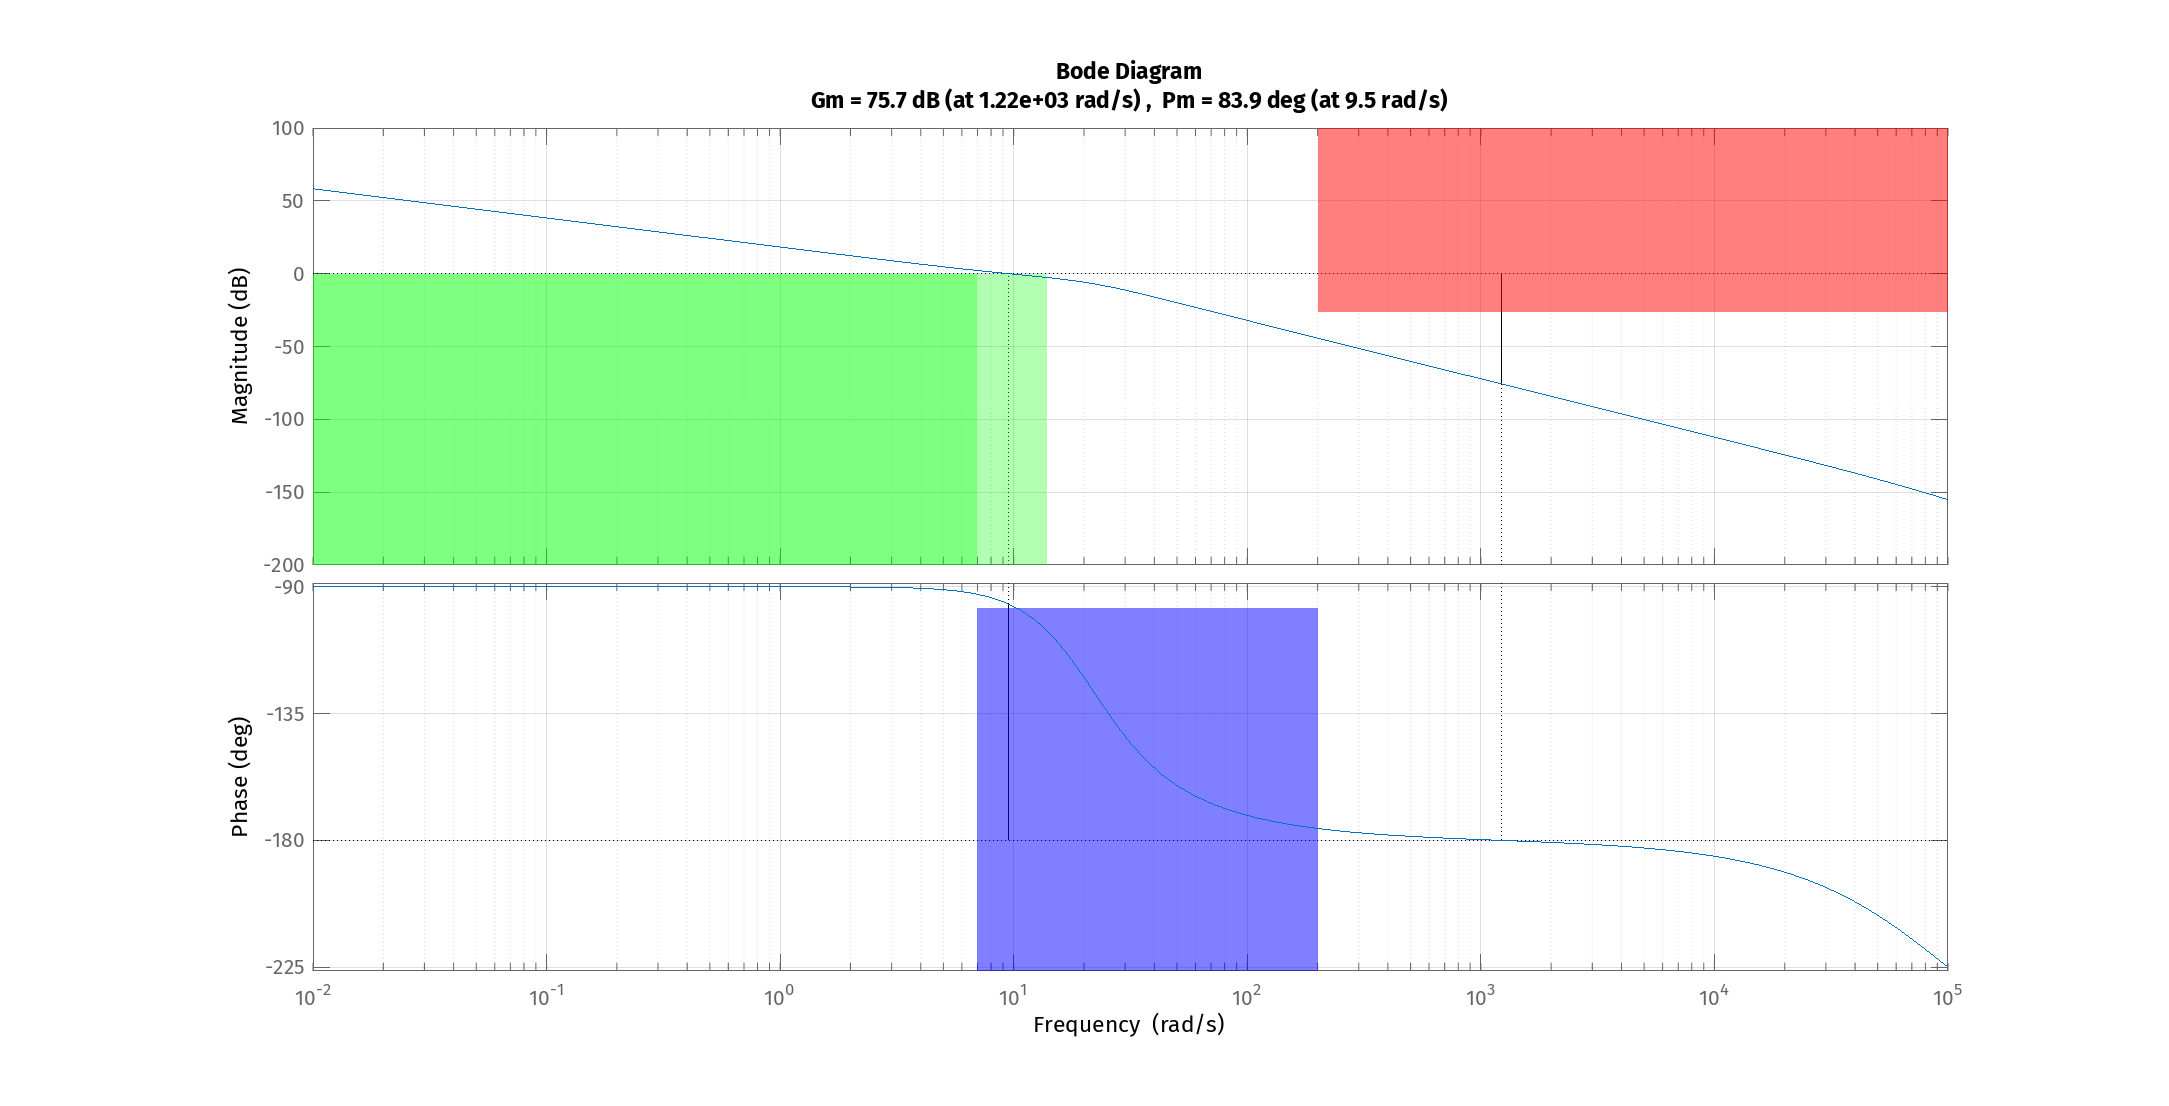
\includegraphics[width=\textwidth]{bode_L_sta}
    \caption{Diagramma di Bode del sistema con regolatore che rispetta le specifiche standard.}
    \label{fig:bode_L_sta}
\end{subfigure}
~
\begin{subfigure}{0.49\textwidth}
    \centering
    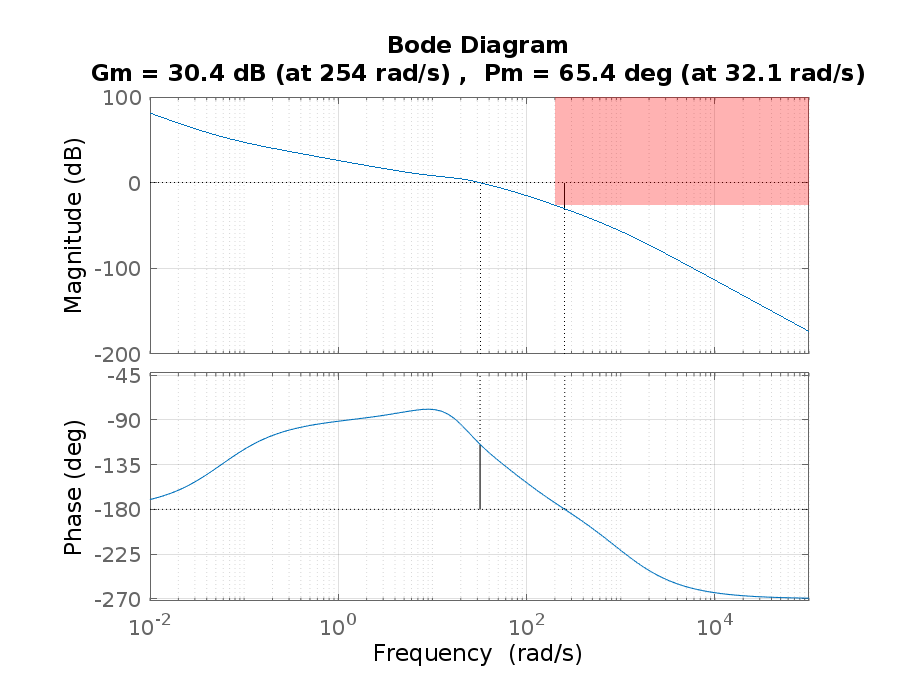
\includegraphics[width=\textwidth]{bode_L}
    \caption{Diagramma di Bode del sistema con regolatore che rispetta le specifiche ottimali.}
    \label{fig:bode_L}
\end{subfigure}
\end{figure}
\section{Risposta del sistema in anello chiuso con regolatore}
Entrambi i regolatori non presentano sovraelongazione quando applicate al sistema linearizzato.
Il regolatore semplice garantisce un tempo di assestamento all'1\% pari a 0.5387 secondi, mentre il regolatore ottimale garantisce un tempo di assestamento all'1\% pari a 0.3817 secondi (misurato con la funzione MATLAB \texttt{stepinfo}).
\begin{figure}[h!]
    \centering
    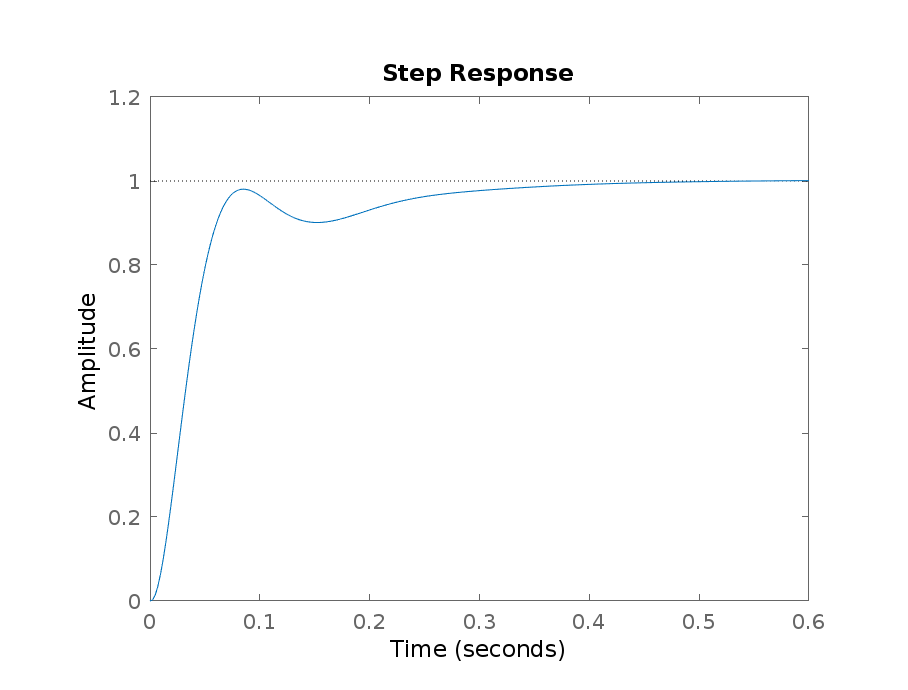
\includegraphics[width=0.55\textwidth]{step}
    \caption{Risposta allo scalino del sistema in anello chiuso con regolatore standard}
    \label{fig:step_standard}
\end{figure}

\subsection{Simulink}
Il sistema è stato simulato, sia nella sua versione linearizzata che in quella non linearizzata, servendosi del pacchetto software Simulink. 
Il sistema non linearizzato è stato realizzato con un blocco "MATLAB Function" che calcola le espressioni nella \cref{eqn:model}, le passa a quattro blocchi integratori e riceve in ingresso il risultato.
Il regolatore ottimale riesce a ottenere buone prestazioni, evidenziate nelle \cref{fig:sim_nonlin} e \cref{fig:step_sim_nonlin}, anche nel sistema non linearizzato.
Si osserva tuttavia che quest'ultimo presenta notevoli divergenze dal sistema linearizzato per i valori di ingresso a scalino richiesti dalle specifiche, rimanendo stabile solo con sollecitazioni almeno otto volte meno intense.
\begin{figure}[h!]
    \centering
    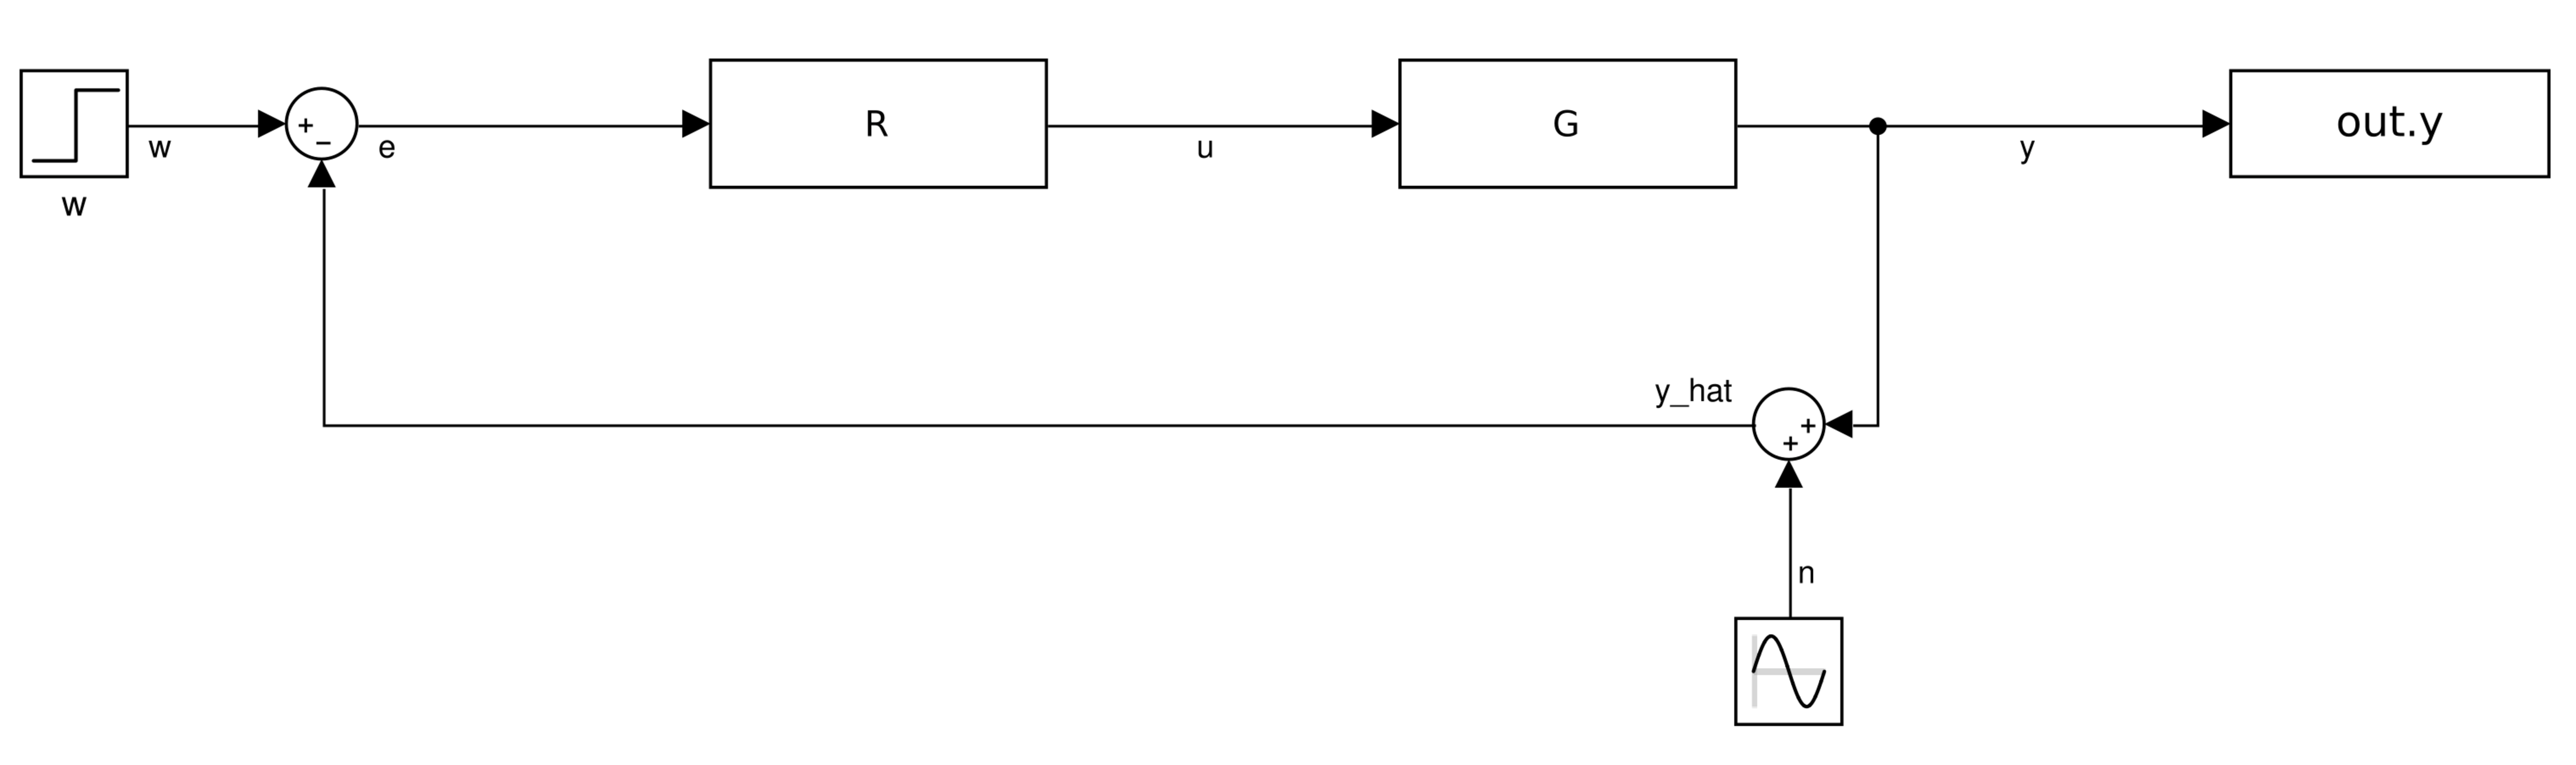
\includegraphics[width=0.7\textwidth]{Simul1C.pdf}
    \caption{Schema Simulink del sistema linearizzato.}
    \label{fig:sim_lin}
\end{figure}
\begin{figure}[h!]
    \centering
    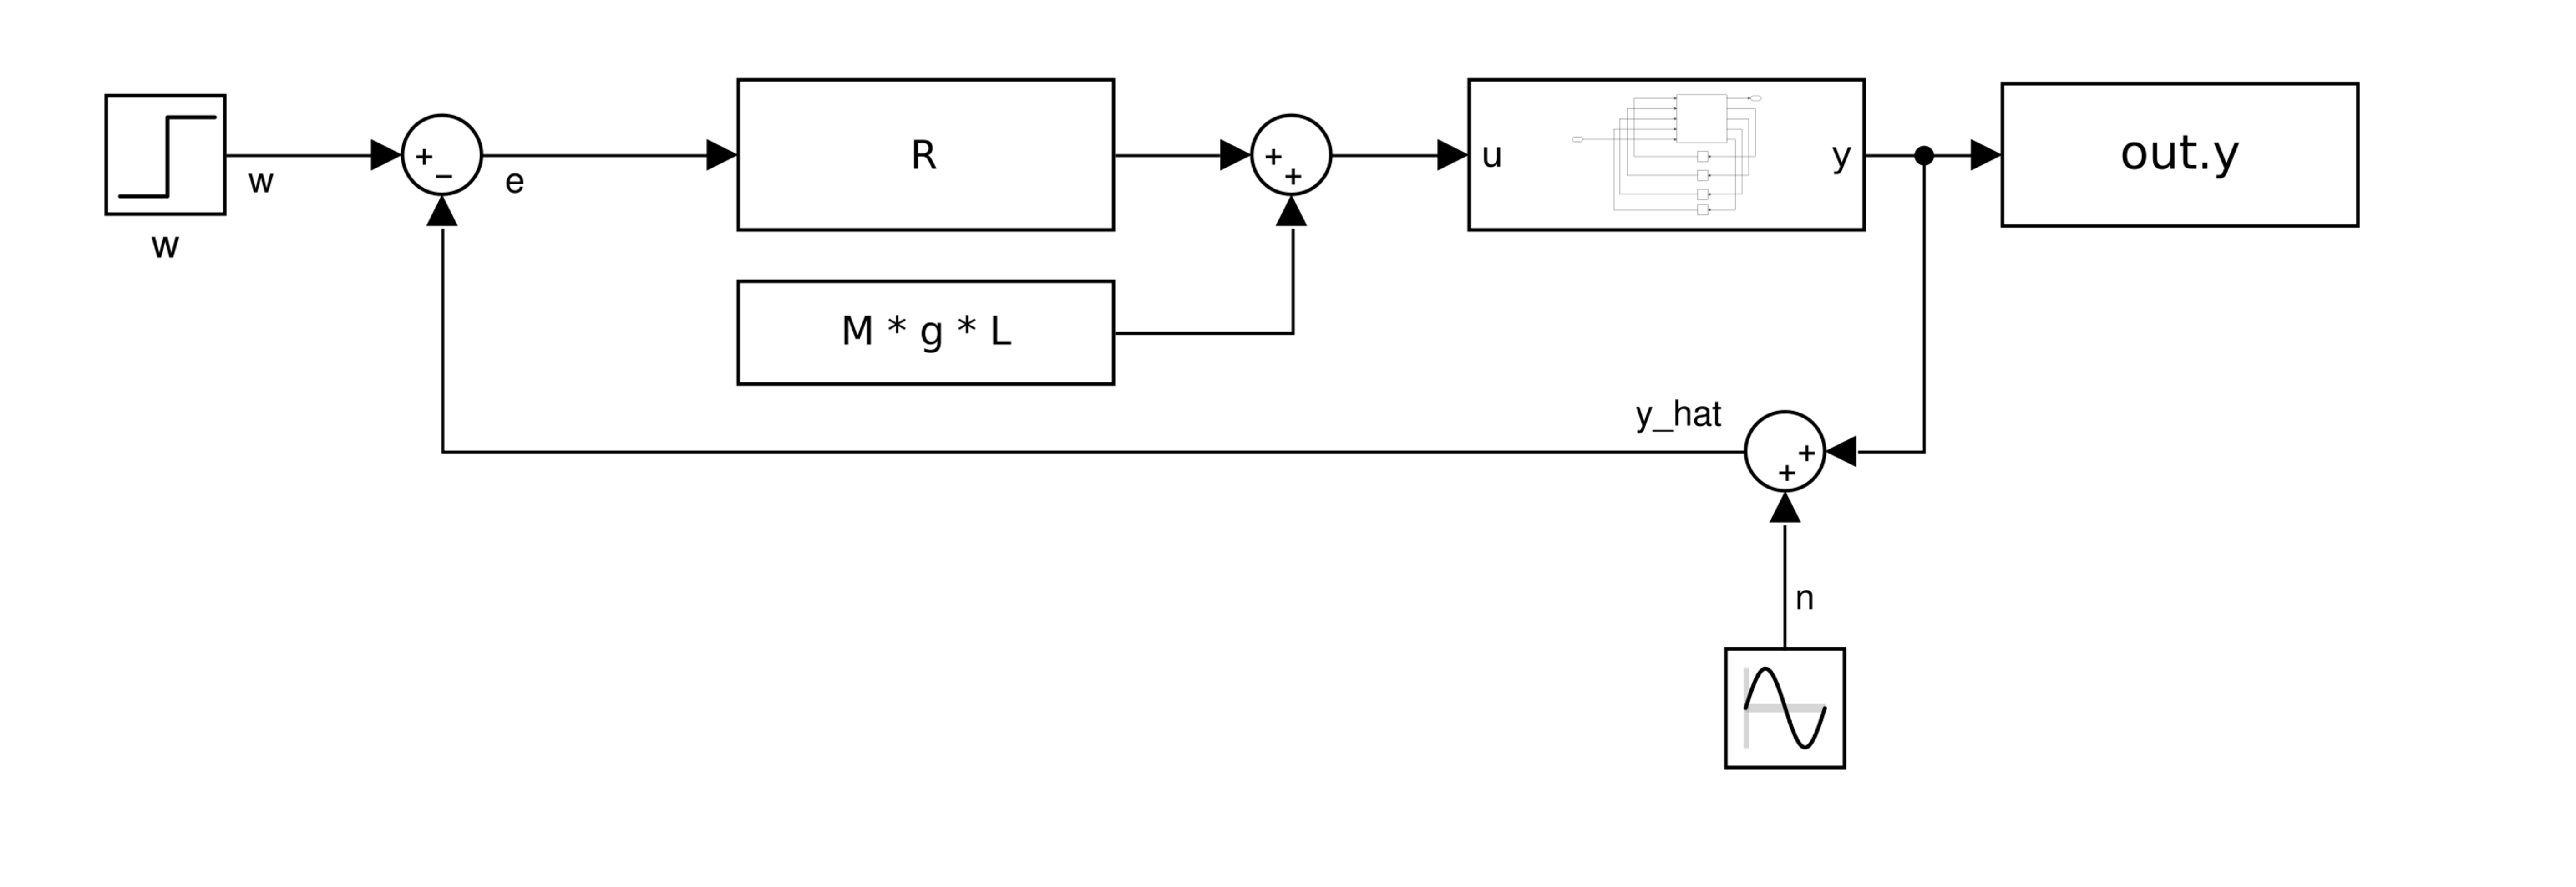
\includegraphics[width=0.7\textwidth]{NonLin1C.pdf}
    \caption{Schema Simulink del sistema non linearizzato. }
    \label{fig:sim_nonlin}
\end{figure}
La risposta allo scalino del sistema linearizzato ricalca quella ottenuta con la funzione \texttt{step} di MATLAB.
La risposta allo scalino del sistema non linearizzato mostra che è possibile ottenere stabilità solamente con valori di ingresso a scalino inferiori a $w = \frac{W}{8} \sca(t)$. 
\begin{figure}[h!]
    \centering
\begin{subfigure}[t]{0.3\textwidth}
    \centering
    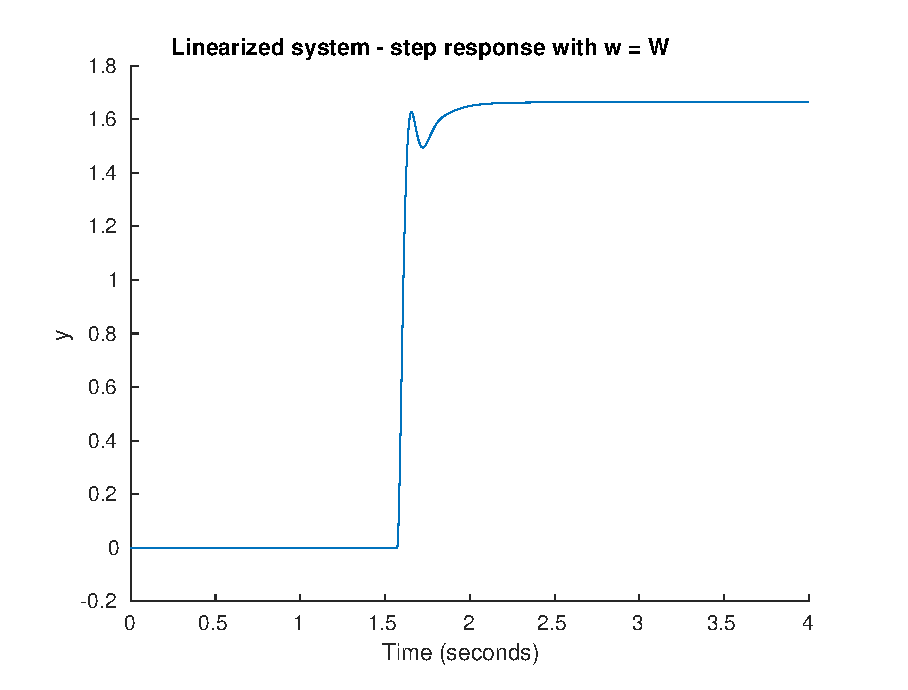
\includegraphics[width=\textwidth]{step_lin}
    \caption{Risposta allo scalino del sistema linearizzato con ingresso $w = W \sca (t)$.}
    \label{fig:step_sim_lin}
\end{subfigure}
~
\begin{subfigure}[t]{0.3\textwidth}
    \centering
    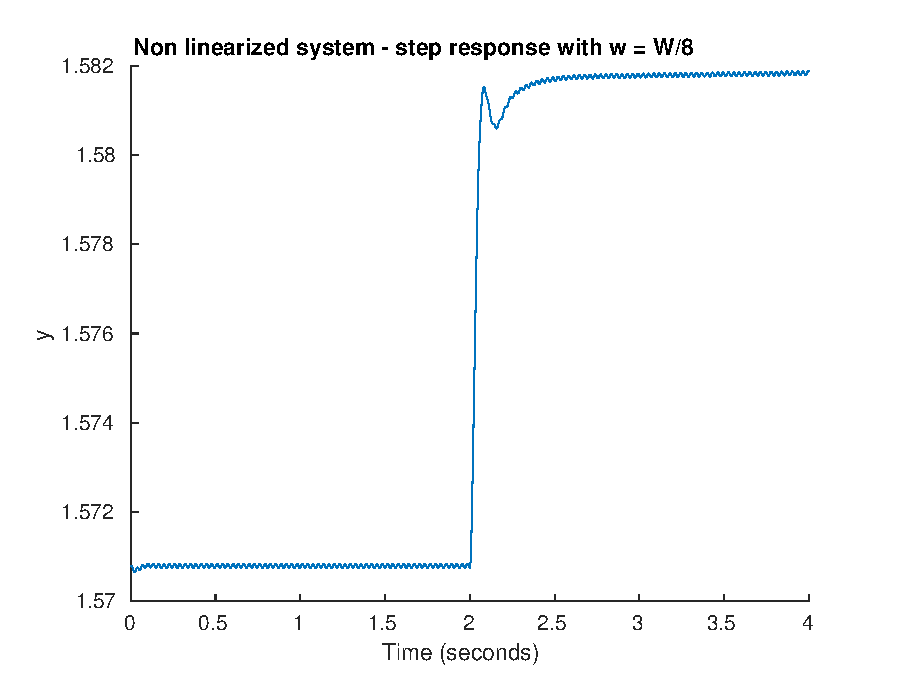
\includegraphics[width=\textwidth]{step_nonlin_short}
    \caption{Risposta allo scalino del sistema non linearizzato con ingresso $w = \frac{W}{8} \sca (t)$.}
    \label{fig:step_sim_nonlin}
\end{subfigure}
~
\begin{subfigure}[t]{0.3\textwidth}
    \centering
    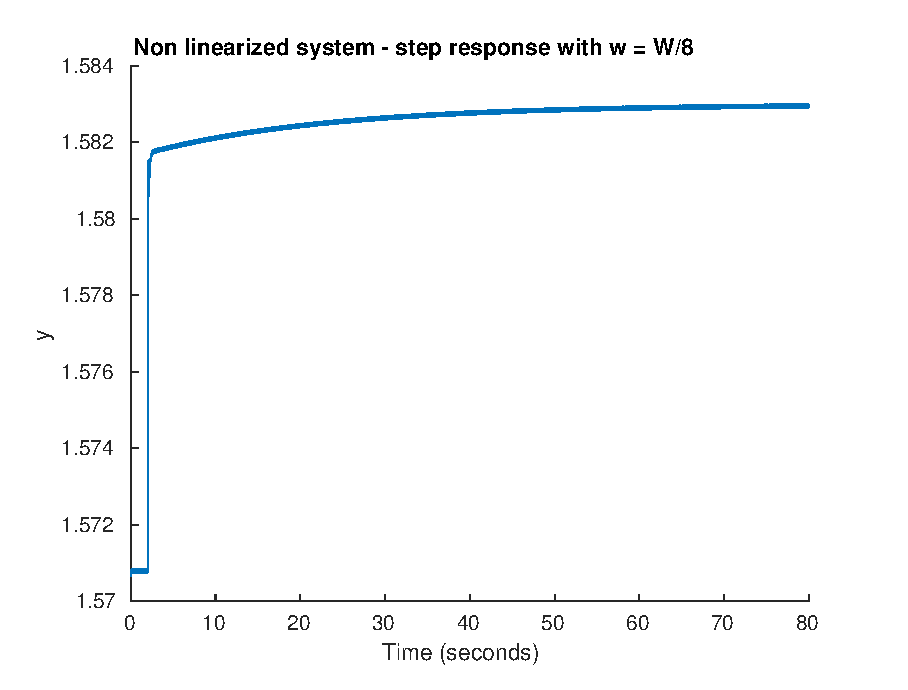
\includegraphics[width=\textwidth]{step_nonlin_long}
    \caption{Risposta allo scalino del sistema non linearizzato con ingresso $w = \frac{W}{8} \sca (t)$ che mostra la lunga coda di assestamento.}
    \label{fig:step_sim_nonlin_long}
\end{subfigure}
\end{figure}
\end{document}